\chapter{Conclusion}
\section{Introduction}
This chapter contains reflections on the work that has been done, how the work process has been done, and what can be done in the future that can strengthen the thesis.

\section{Reflection}


\section{The Work Process}

\subsection{Meetings}
The team held meetings with their supervisor, Filip Holik, on a weekly basis. Although the meetings were typically scheduled for Wednesdays, they had to be postponed or canceled on occasion due to various circumstances. Meeting Minutes with the supervisor can be found in Appendix \ref{supervisormeeting}.
\\~\\
During the early stages of the project, the team met with the stakeholder every other week. However, as the project progressed, both parties agreed that weekly meetings would be beneficial. As the demand for help grew, the group required more regular assistance. Meeting Minutes with the stakeholder can be found in Appendix \ref{nbimmeeting}.  



\subsection{Scrum}
Throughout the thesis, the group followed the Scrum framework of agile project management, which required breaking the project down into a series of sprints lasting two to four weeks. To keep everyone informed, daily stand-up meetings were held, during which members delivered progress reports on the thesis and discussed plans for the day, including each member's allocated chores. While the group aimed to meet daily, this was not always possible because some members had work obligations in addition to their studies.
\\~\\
Despite this, the team had sprint planning and retrospective sessions every two weeks to review progress and establish goals for the next two weeks. During the retrospective meetings, the team engaged in self-reflection by asking questions such as "What should we keep doing?" "What should we do more of?" "What should we do less of?" and "What should we stop doing?" in order to identify areas for improvement for the next sprint cycle. During the sprint planning meetings, on the other hand, the group evaluated completed tasks and discussed what needed to be done before the next sprint period.
\\~\\
The meetings were originally set for Fridays, but the group realized that conducting them on Mondays would be more effective. This is because starting a new strategy at the beginning of the week is more successful than beginning a new plan at the end of the week.
\\~\\
Following the Scrum framework helped in the promotion of good communication and teamwork among group members. Furthermore, the Kanban board was integrated into the Scrum Framework and proved to be quite useful in tracking tasks that were ongoing, completed, or yet to be started. When a member of the group completed a task, there were always tasks on the Kanban board that needed to be completed. 


\subsection{Coordinated schedule}
Because the team members were involved in other activities such as jobs and involvement in the student association, it was important for them to coordinate their schedules. This method allowed the team to organize meetings more effectively and determine each member's availability for work. The team scheduled all of their activities and workdays using the calendar feature of their Teams channel.

\subsection{Draft Submissions}
The team set specified deadlines for producing multiple drafts at the start of the project. This approach tried to maintain constant development while avoiding last-minute delays. For instance, the group set an April 1st target for their first draft, which they were able to meet. As a result, both the supervisor and the stakeholder received the first draft on time. After a few days, the team got feedback and proceeded with their work. 
\\~\\
The team established a deadline for the final draft. In order to give the supervisor and stakeholders enough time to thoroughly read the thesis before the submission date on the 22nd of May, the team established the deadline for the final draft on the 1st of May, three weeks before the submission date. 


\subsection{Gantt Chart}
Since the group decided to do some changes to the scope during the project period, the original Gantt chart could not be followed. 
\\~\\
The research on tools was considered to be time-consuming at first, but with the changes made, this activity ended up being a smaller part of the thesis than anticipated. As a result, it took less time than what was first estimated. Furthermore, the \say{Testing tools} activity was removed since the team wanted to focus less on testing tools and more on integrating testing of the various tools into the pipeline-building process. 
\\~\\
The process of learning \acrshort{aws} and configuring the pipeline with Terraform took longer time than initially expected.
The documentation for \acrshort{aws} and Terraform is extensive, but it can be overwhelming to navigate. With so many different services and features offered by \acrshort{aws}, the group had to determine which ones were the best fit for their needs. Building the pipeline required a significant amount of functionality to be in place for additional features to work properly. 
\\~\\
However, the group managed to follow the planned deadlines for the different draft submissions. The first draft was delivered on the 3rd of April in week 13, and the final draft on the 5th of May in week 18. 

\vspace{2mm}
\begin{figure}[H]
    \centering
    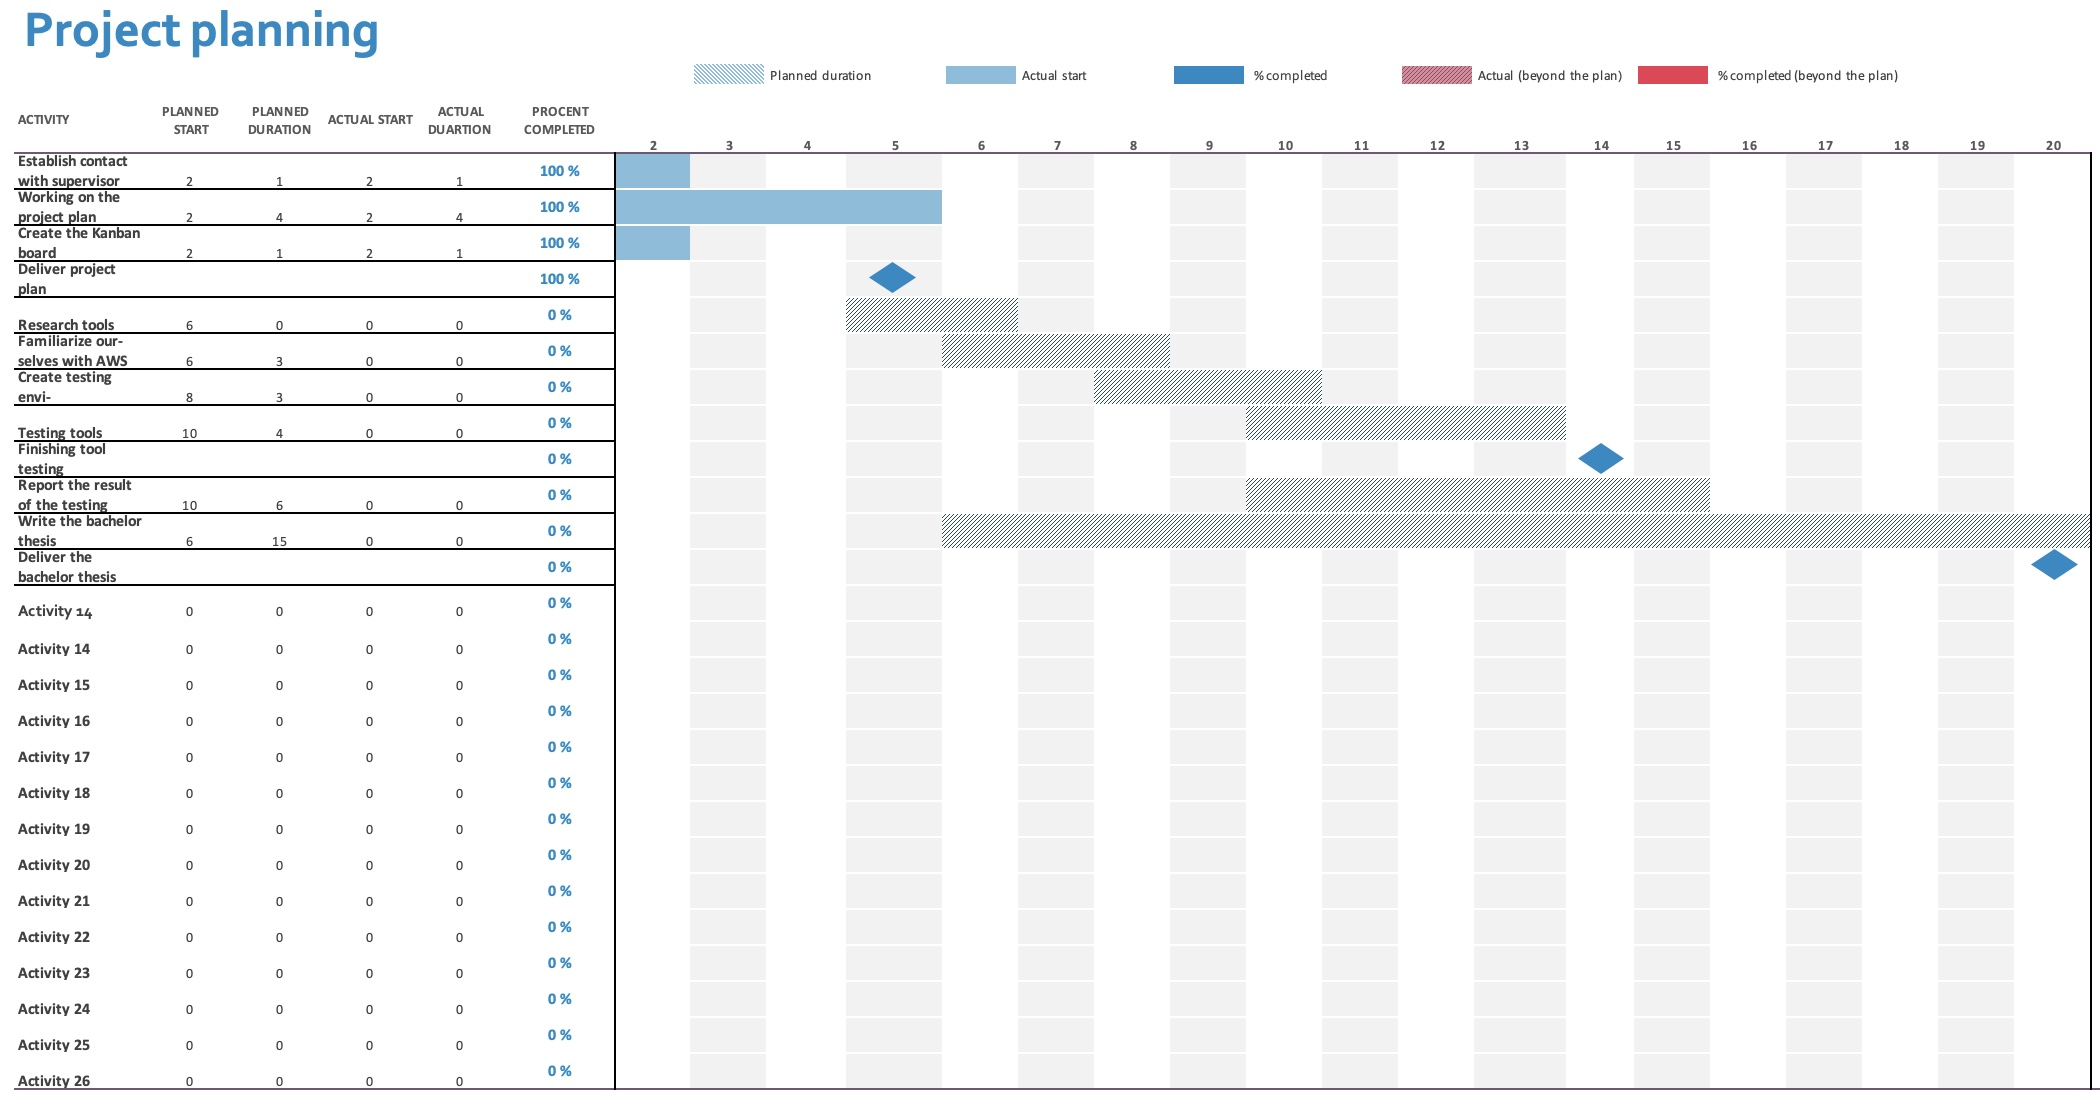
\includegraphics[width=1\columnwidth]{Images/gantt2.jpg}
    \caption{Original Gantt Chart}
    \label{fig: Original Gantt Chart}
\end{figure}

\vspace{2mm}
\begin{figure}[H]
    \centering
    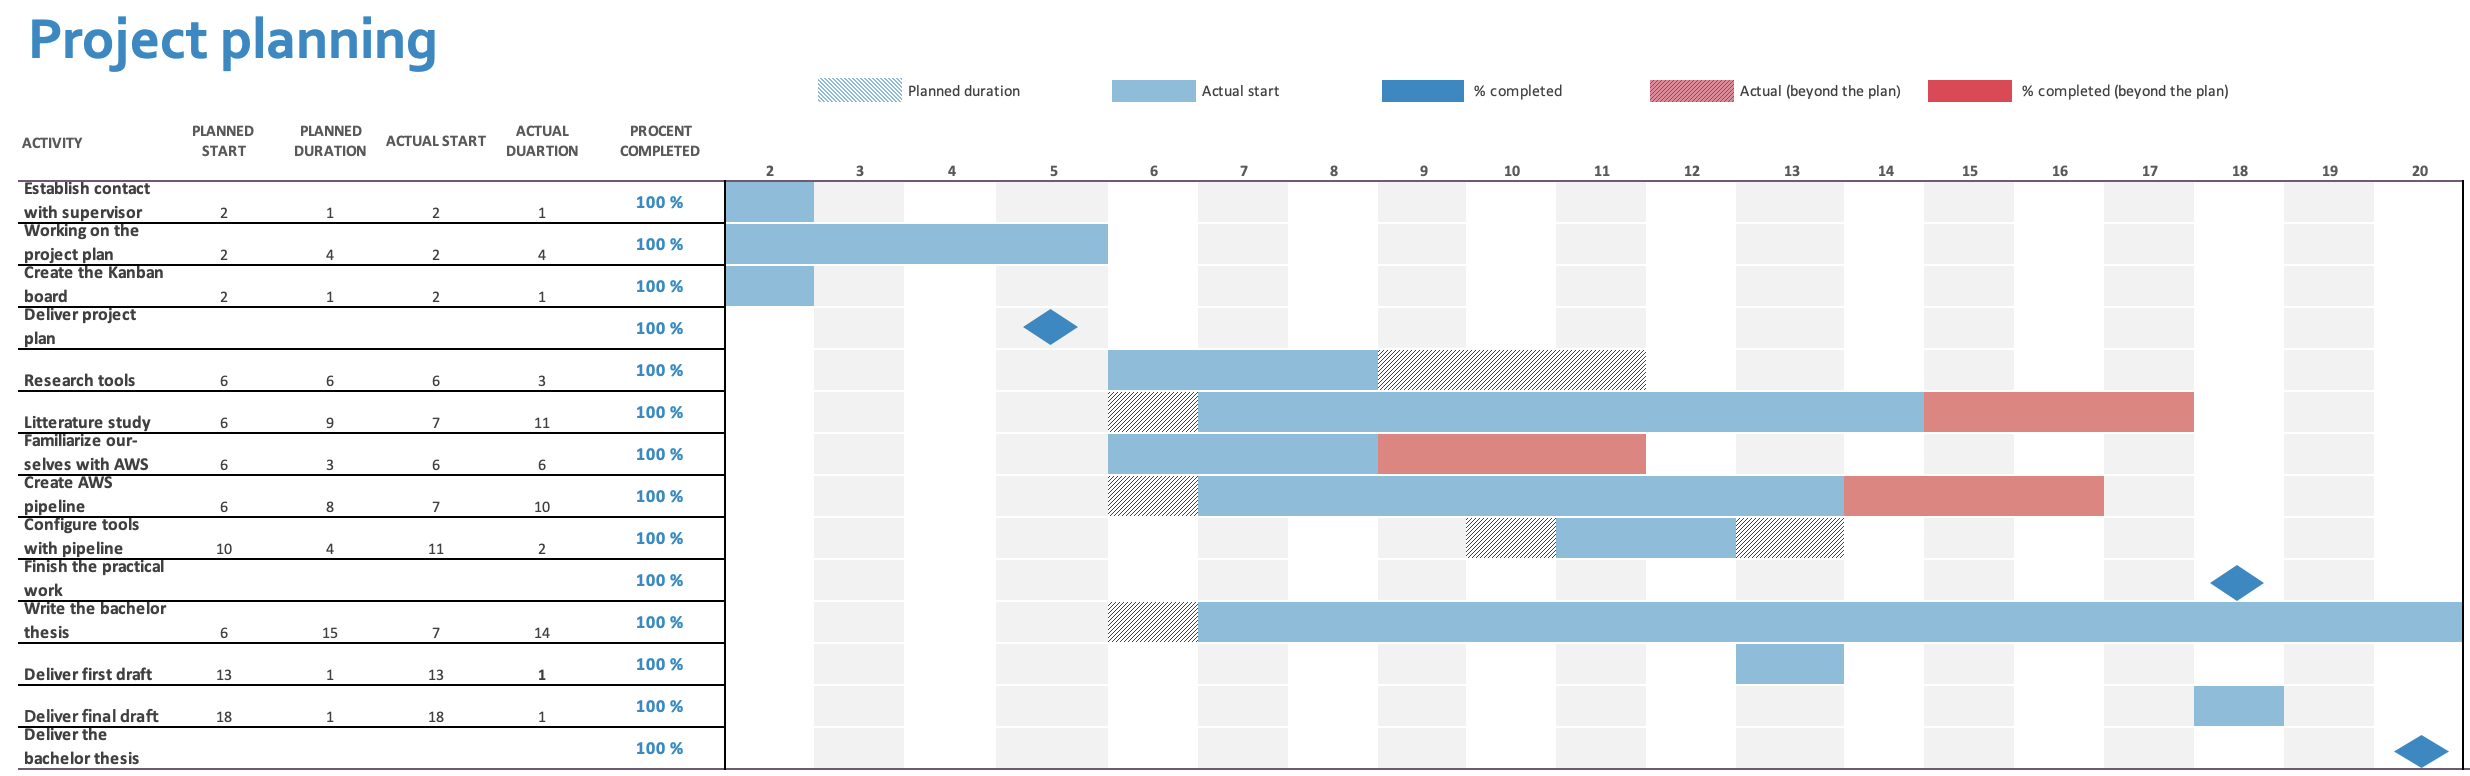
\includegraphics[width=1\columnwidth]{Images/finished-gantt.png}
    \caption{Updated Gantt Chart}
    \label{fig: Updated Gantt Chart}
\end{figure}


\subsection{Distribution of Work}
The group decided to divide the work into two parts at the start of the thesis to ensure that the thesis progressed continuously. The first part is practical, and the second is report writing. The responsibilities were assigned based on each group member's strength and what they most desired to do. Every member of the group contributed to the thesis, and everyone worked together to complete the report on time. 


\subsection{Goals}
P1: \textit{Collaborate effectively with team members to ensure the timely completion of tasks}, was achieved. As stated previously, the group incorporated a Kanban board into the Scrum framework allowing for the assignment and tracking of tasks. Additionally, the group utilized various communication platforms, such as Discord and Teams, to ensure effective communication among the group members. It was important to use communication tools that were already integrated into each member's daily workflow, and these two platforms proved to be the most effective for the team´s needs. 
\\~\\
P2: \textit{Successfully integrate security tools (e.g., SAST, DAST, SCA) into the SDLC pipeline}, was achieved. The group found tools that could be integrated into the pipeline between GitHub and AWS to secure the application code that´s being sent through.
\\~\\
P3: \textit{Implement an automated pipeline using Terraform to build, test, and deploy applications}, was achieved. The group created Terraform code that automated the pipeline, from the build to the deployment. 
\\~\\
R1: \textit{Develop a secure and automated pipeline for the SDLC process using Terraform}, partially achieved. The group developed an automated pipeline using Terraform code and implemented restricted access management to ensure pipeline security. However, it would be presumptuous to claim that the pipeline is 100\% secure, as the group did not have sufficient time to implement signed artifacts. This would have ensured that the code pushed to the GitHub repository was the same as the code being sent through the pipeline, thus guaranteeing code integrity. Consequently, while the pipeline can be deemed secure, the group cannot be completely certain that the code sent through is secure. Hence, the goal of achieving a complete, secure, and automated pipeline remains partially fulfilled. 
\\~\\
R2: \textit{Produce a report summarizing the results of the project and recommendations for improving the SDLC pipeline security}, was accomplished to a certain degree. The resulting report provides numerous essential and effective practices that can be implemented to improve security in the \acrshort{sdlc}. Despite this, some sections, particularly the practical section, may be lacking in proper safety measures. Since the group did not write the application code, they were unable to follow best practices for code-writing, which is an important step that is not covered in this thesis.   



%R3: \textit{Provide a comprehensive analysis of how a secure pipeline can be built from GitHub to AWS. }

%R4: \textit{Offer new insights and perspectives on the topic, which can increase the stakeholder's awareness of the different topic areas. }



\section{Further Work}
In further work, it could strengthen the thesis to perform a broader analysis of various security tools that perform SAST, DAST, and SCA scans -  where the selected tools are based on these analyses. During these analyses, an assessment can also be made of which requirements must be met in order for a tool to be selected. 
\\~\\
It would have been beneficial to include earlier phases in the thesis to acquire a more thorough grasp of the entire \acrlong{sdlc} and adhere to the shift-left methodology, which emphasizes early testing to find vulnerabilities earlier. This would have illustrated the shift-left method of undertaking testing as early as possible in the process.  
\\~\\
Although the group was primarily focused on automating the practical processes, there were some challenges. Despite the group's efforts, they were not able to fully automate the process of enabling Dependabot and Secret Scanner from the \acrshort{cli}. The complete automation of the pipeline could have been achieved to a greater extent by automating these tools. 

\section{Conclusion}
%snakke om hva vi har gjort og hva vi anbefaler 